\chapter{Análisis e interpretación del mapa de comportamientos}\label{cha:labels}

Una vez obtenida la segmentación del mapa de t-SNE, nos propusimos analizar si los \textit{labels} obtenidos se corresponden con determinados comportamientos o poses del animal observables por el experimentador, es decir, si podemos interpretar el mapa obtenido. Dado que t-SNE es un algoritmo de clasificación no supervisada, es posible que algunos o todos los \textit{labels} obtenidos no sean interpretables. En este capítulo estudiaremos las propiedades del mapa de comportamientos obtenidos en el Capítulo \ref{cha:mapa}. También analizaremos las propiedades de los \textit{labels} obtenidos a partir de la segmentación del etograma y los interpretaremos como poses específicas adoptadas por los ratones expertos durante la ejecución de la tarea \textit{rotarod} con aceleración.

A continuación damos un resumen del contenido de este capítulo. Primero, en la Sección \ref{sec:inter_labels} daremos significado a los \textit{labels} que surgieron de la segmentación del etograma. Luego, en la Sección \ref{sec:diversidad} estimaremos la representatividad de cada clase de \textit{labels} dentro del conjunto de ratones individuales. Después, en la Sección \ref{sec:vel_rotarod} caracterizaremos la estadística de las secuencias de \textit{labels} y su dependencia con la velocidad del cilindro \textit{rotarod}. Finalmente, en la Sección \ref{sec:logo} representaremos las secuencias de \textit{labels} como logos de secuencias condicionadas a la ocurrencia de una determinada clase de \textit{label}.

\section{Interpretación del mapa}\label{sec:inter_labels}

Como primera medida nos interesa interpretar los \textit{labels} que surgieron de la segmentación del mapa de comportamientos de la Figura \ref{fig:tsne_labels}. Esto es, interpretar la clasificación no supervisada del comportamiento animal producida utilizando el algoritmo t-SNE. Para ello se compilaron los intervalos de video donde ocurría un \textit{label} determinado por ratón y por \textit{trial}, de manera de poder visualizar la similitud en el comportamiento asociado a cada \textit{label} (\href{https://youtube.com/playlist?list=PLRCempM9WkGZvXhkziQ5Hk8FQTWqDjYet}{\textbf{\textit{link} al material suplementario}}).

Además, la Figura \ref{fig:poses} muestra ejemplos representativos de los fotogramas extraídos. Notablemente, logramos interpretar los \textit{labels} de la segmentación del etograma como diferentes tipos de poses que los ratones adoptan durante la ejecución de la tarea. Por ejemplo, el \textit{label} 2 (7) estaría asociado a una pose asimétrica en la que el ratón da un paso con su pata derecha (izquierda). Por otro lado, los \textit{labels} 5, 6 y 9 estarían asociados a poses simétricas y podrían ser diferentes poses intermedias entre dos pasos consecutivos del ratón o momentos en los que el ratón avanza o salta de manera sincronizada con ambas patas. Por su parte, el \textit{label} 1 (8) podría estar asociado a poses en las que el ratón oculta su pata derecha (izquierda). Por último, las poses asociadas a los \textit{labels} 3 y 4 no fueron interpretadas. En conclusión, la clasificación del comportamiento obtenida nos permite identificar poses individuales del animal de corta duración mientras realiza la tarea.

\begin{figure}[!htbp]
\begin{tabular}{ccc}
\centering
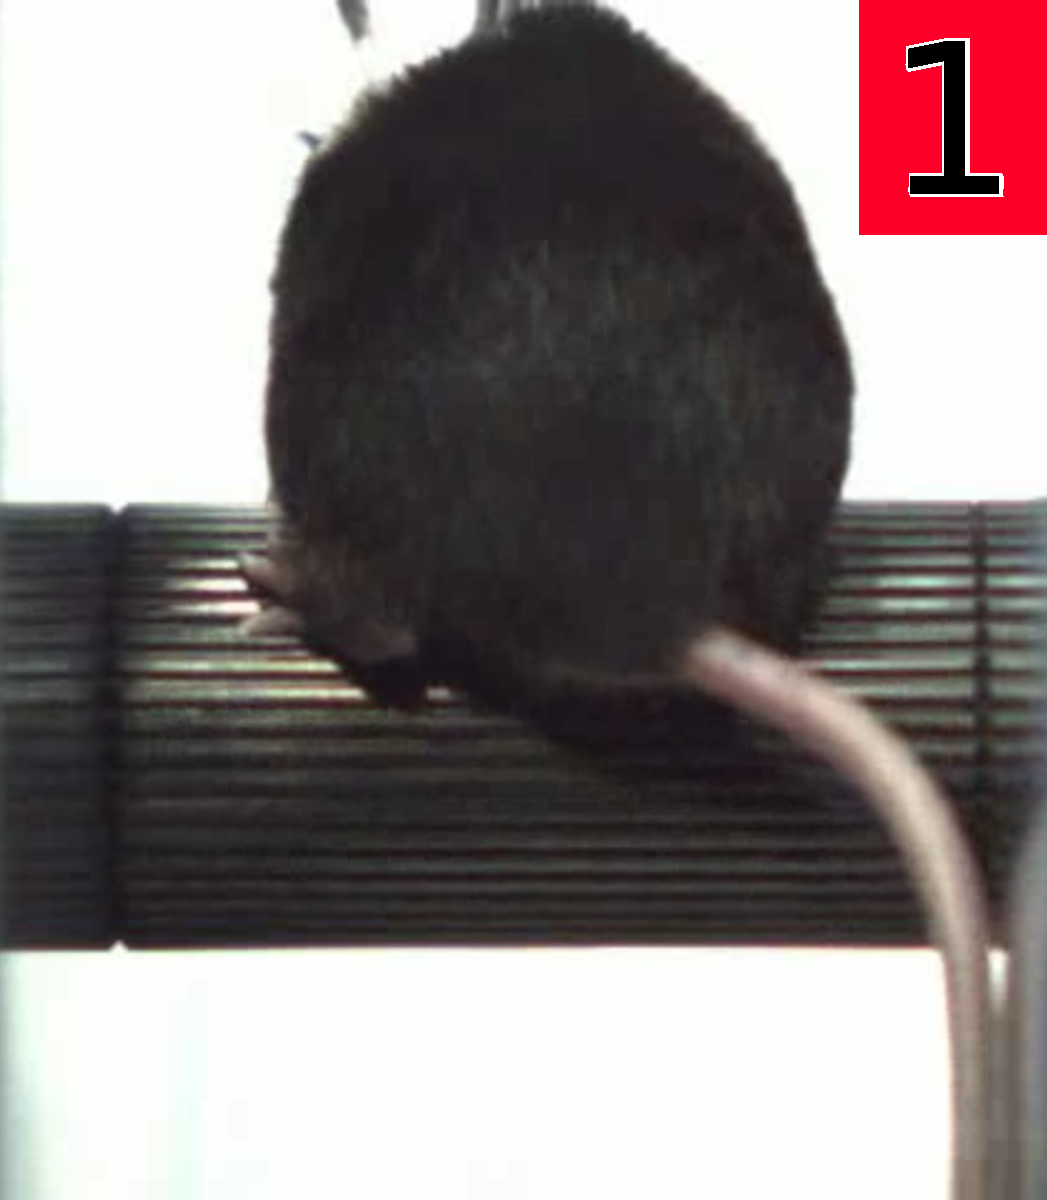
\includegraphics[width=0.32\textwidth]{figuras/expertos/videos/1.pdf} & 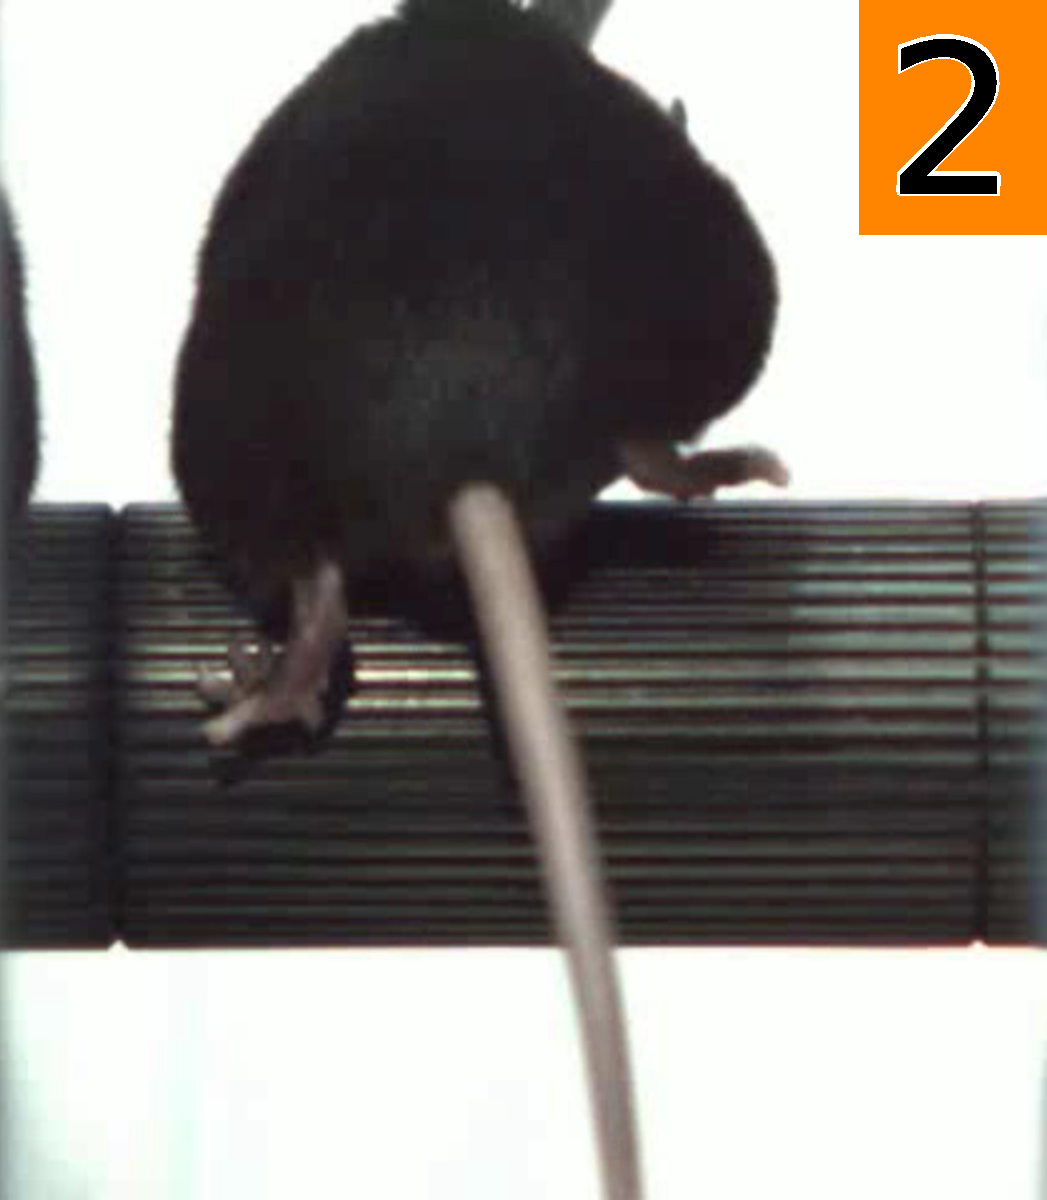
\includegraphics[width=0.32\textwidth]{figuras/expertos/videos/2.pdf} & 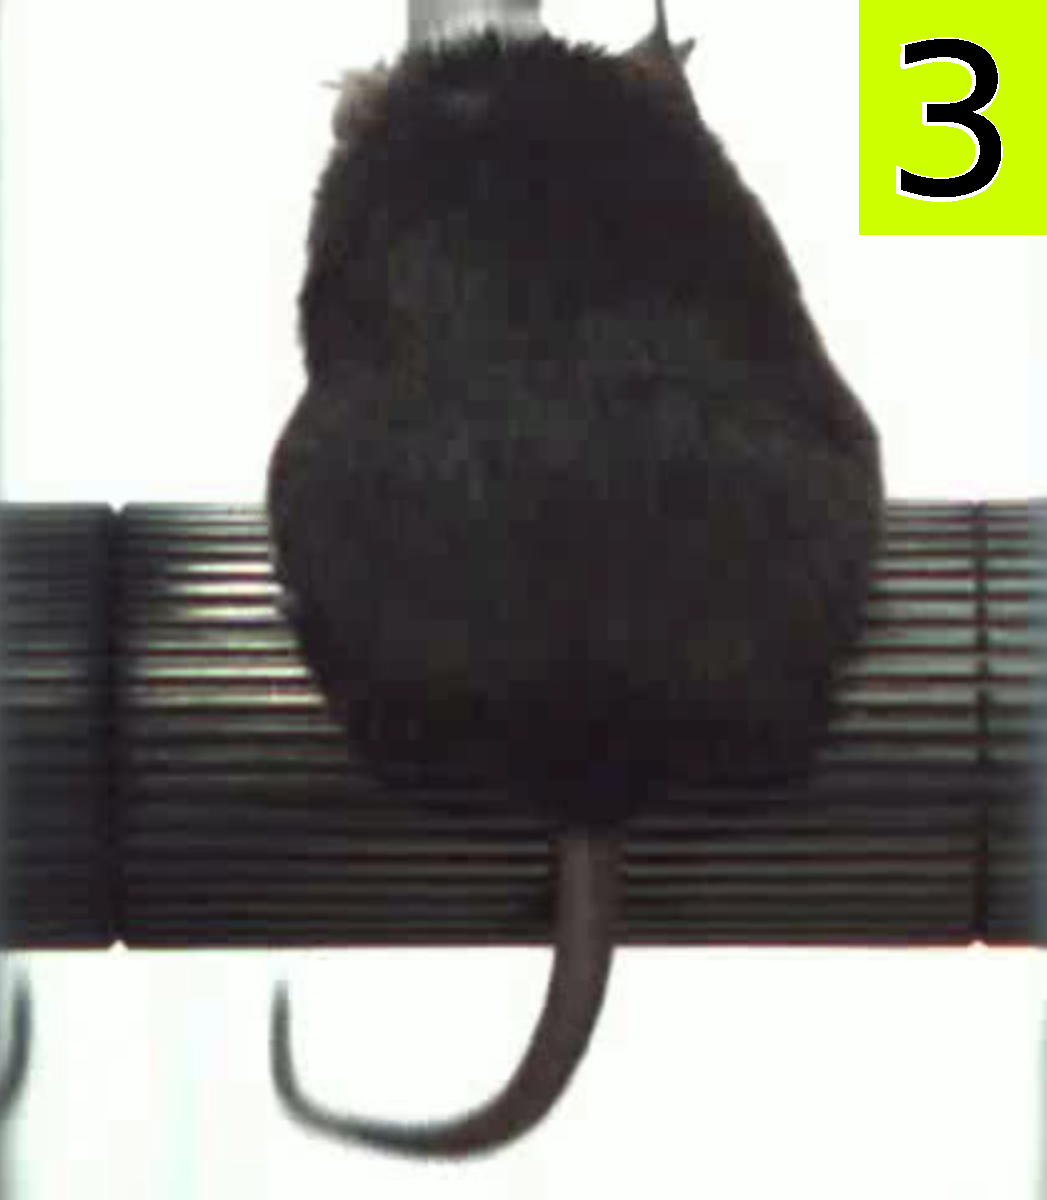
\includegraphics[width=0.32\textwidth]{figuras/expertos/videos/3.pdf} \\
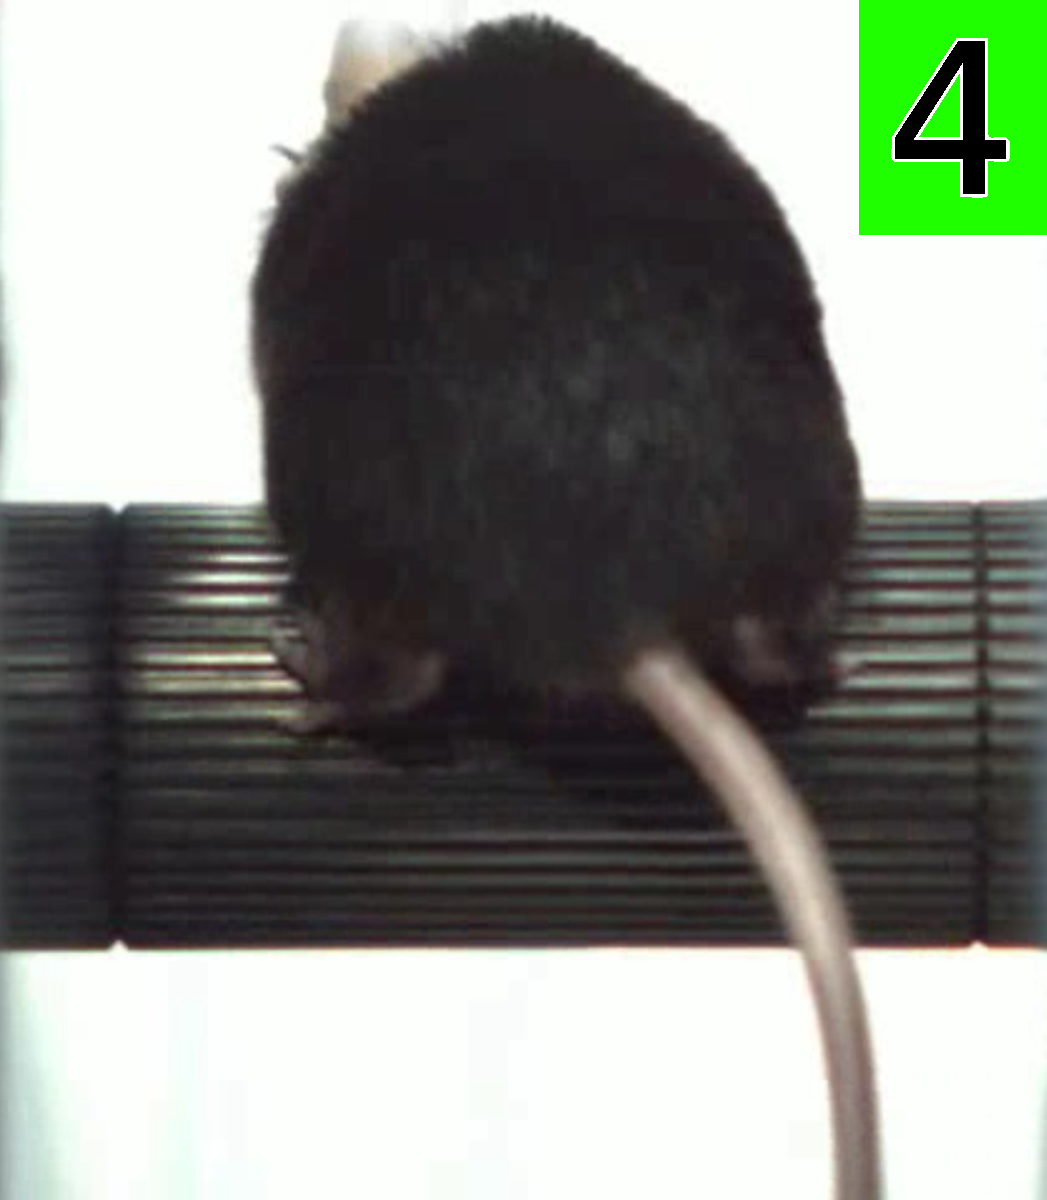
\includegraphics[width=0.32\textwidth]{figuras/expertos/videos/4.pdf} & 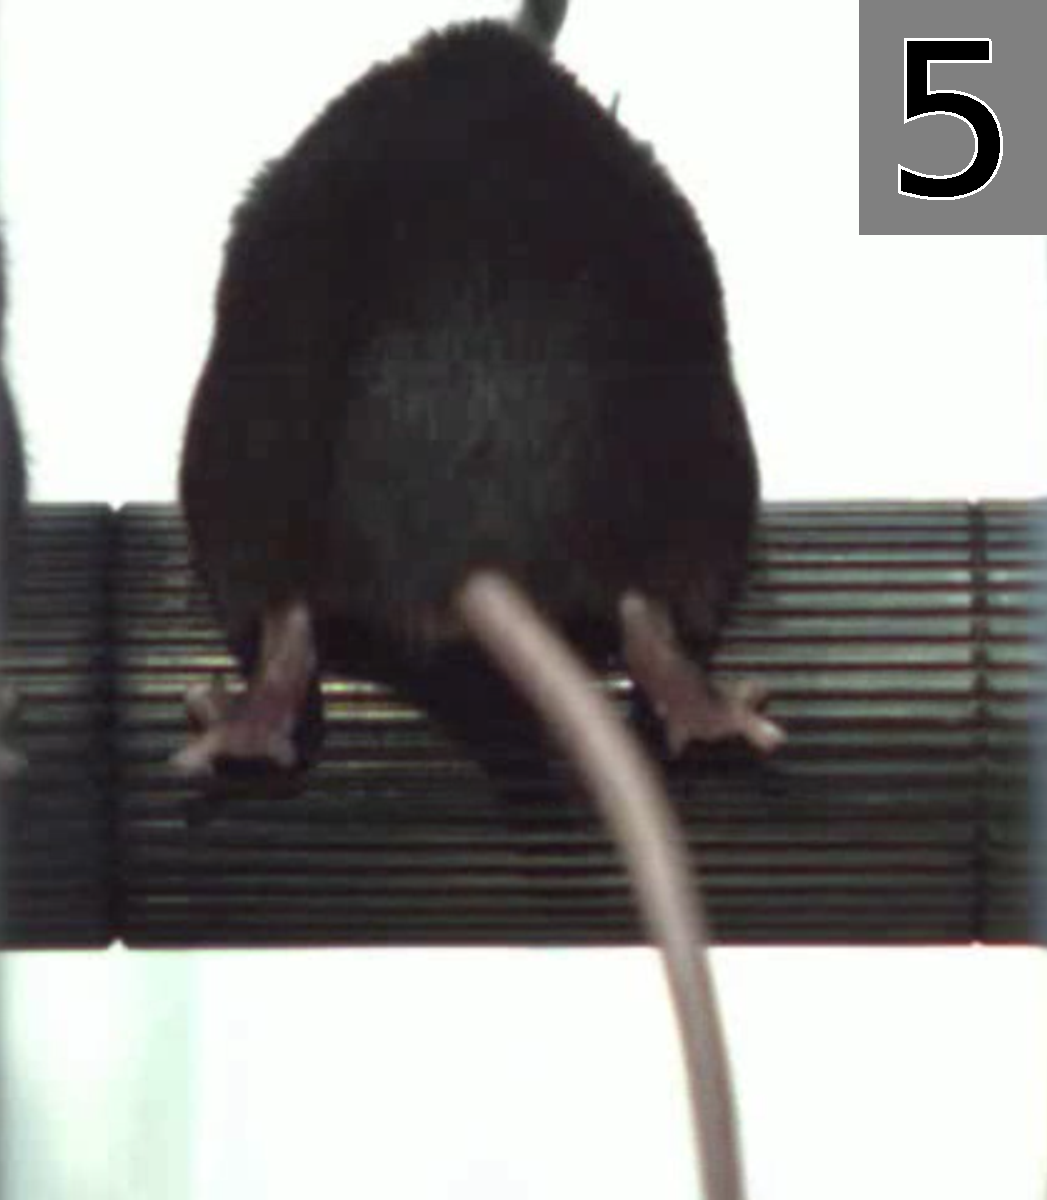
\includegraphics[width=0.32\textwidth]{figuras/expertos/videos/5.pdf} & 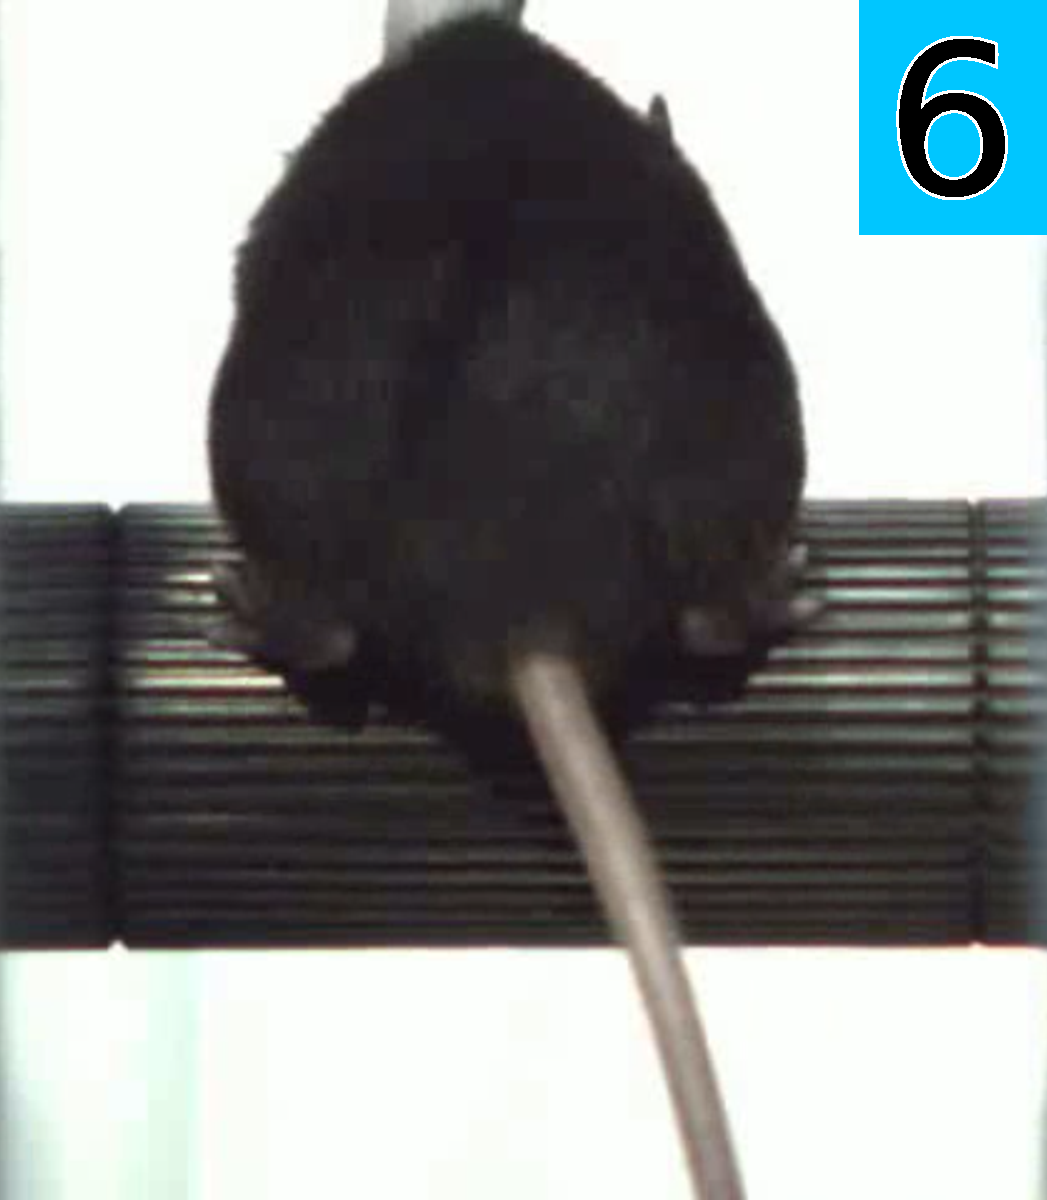
\includegraphics[width=0.32\textwidth]{figuras/expertos/videos/6.pdf} \\
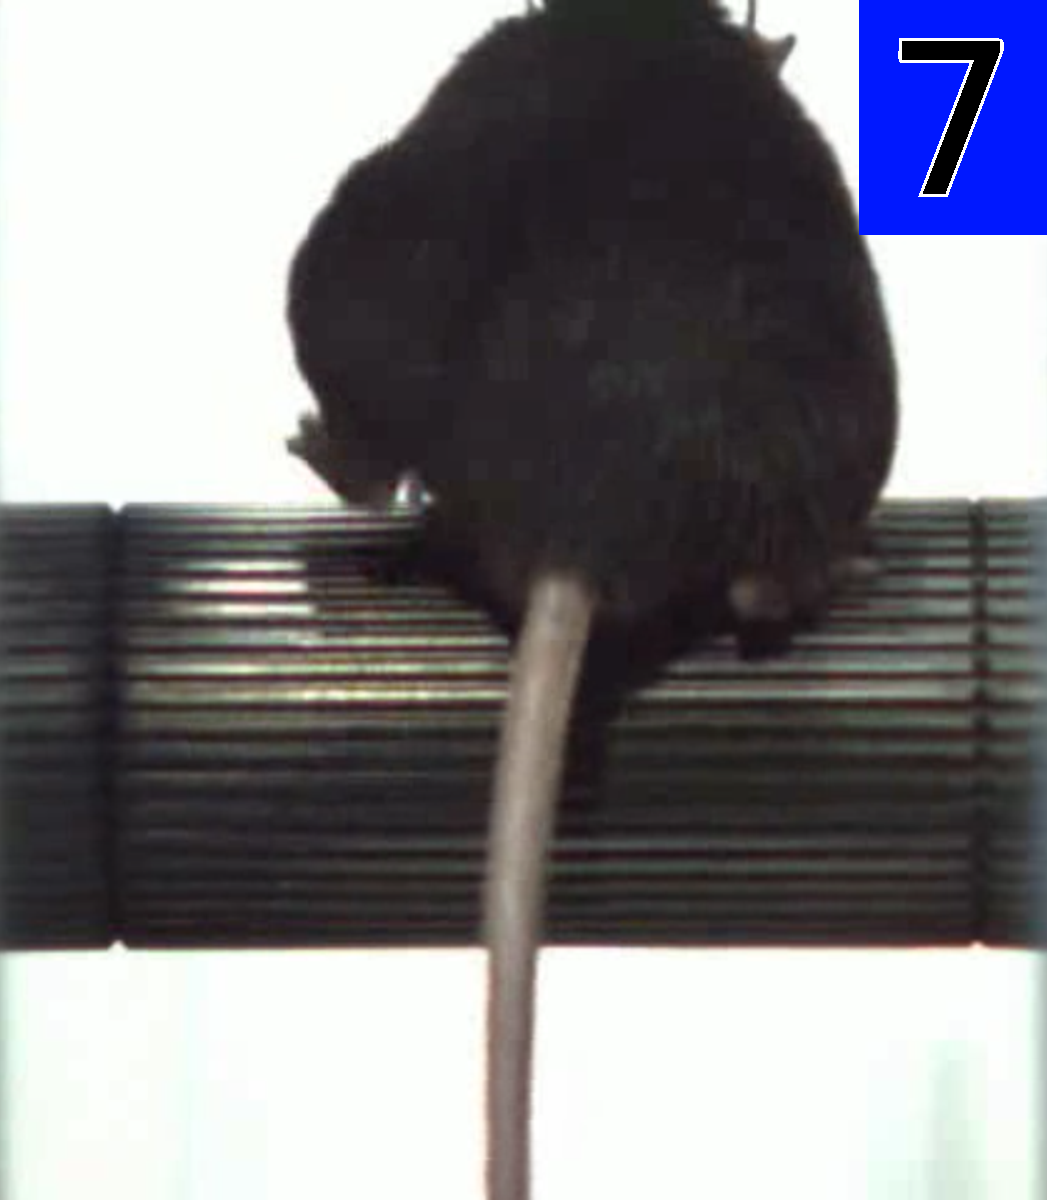
\includegraphics[width=0.32\textwidth]{figuras/expertos/videos/7.pdf} &
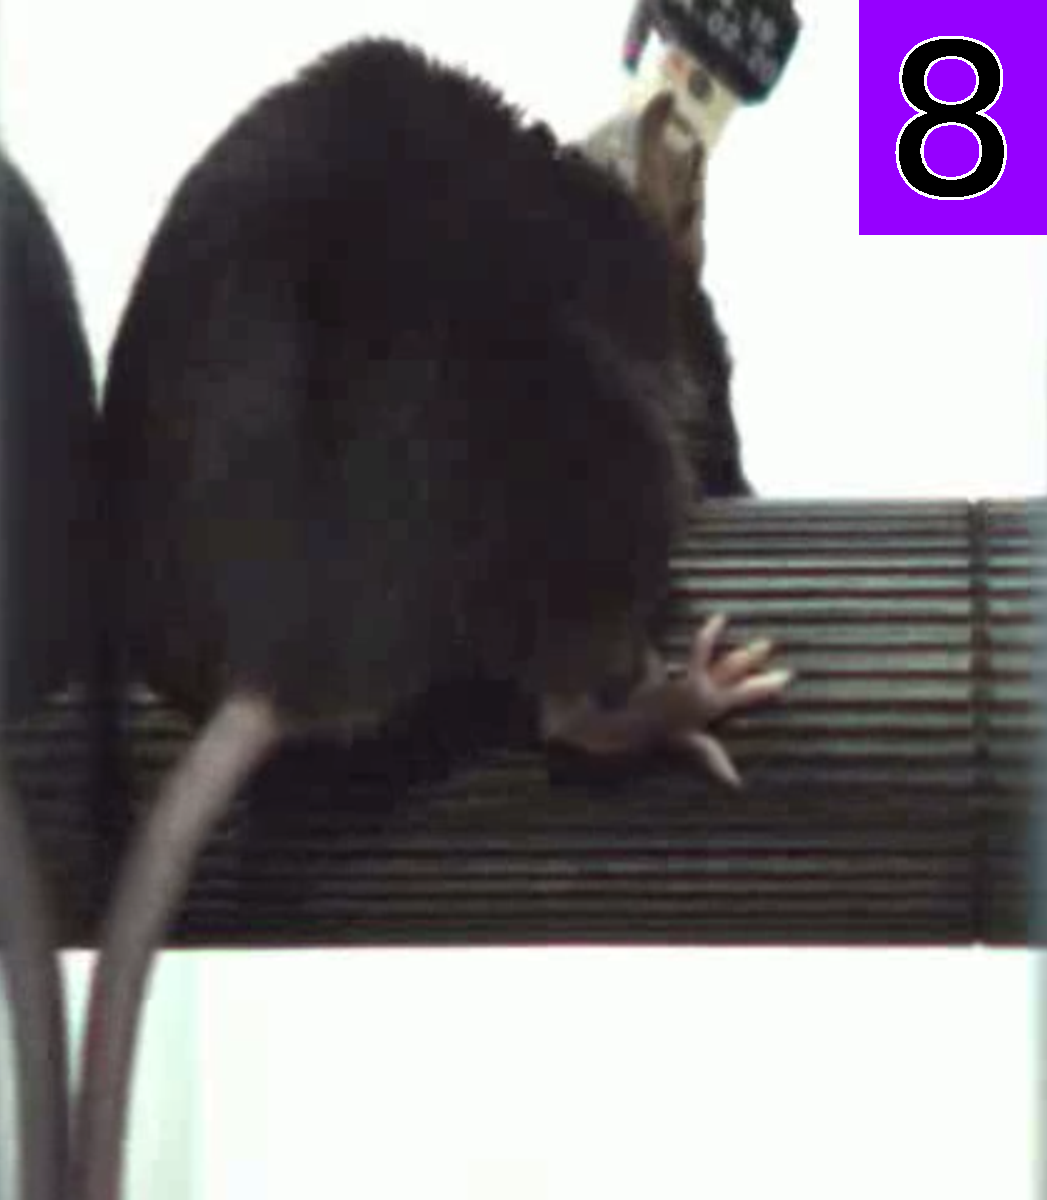
\includegraphics[width=0.32\textwidth]{figuras/expertos/videos/8.pdf} &
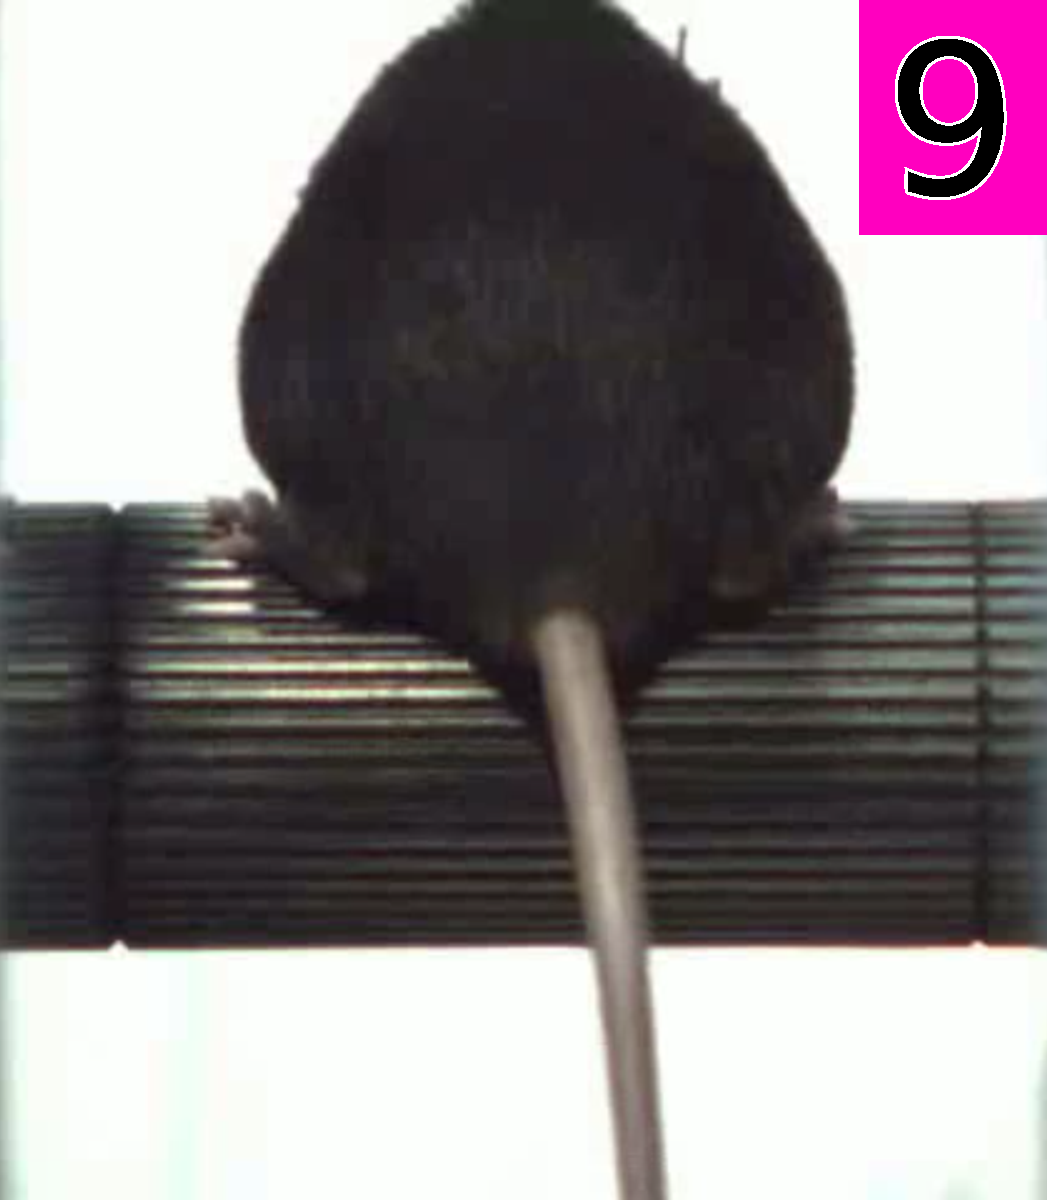
\includegraphics[width=0.32\textwidth]{figuras/expertos/videos/9.pdf}
\end{tabular}
\caption{Fotogramas típicos extraídos de los videos de los ratones expertos durante la realización de la tarea \textit{rotarod}. Se extrajo un fotograma representativo por cada clase de \textit{label}, obtenido a partir de la segmentación del mapa de comportamientos de la Figura \ref{fig:tsne_labels}.}
\label{fig:poses}
\end{figure}

Por su parte, la Figura \ref{fig:label_evento_secuencia} muestra una sucesión típica de \textit{labels}, durante un intervalo de tiempo de 10 s, comenzando a los 10 s de una prueba \textit{rotarod}. En la parte superior de la Figura \ref{fig:label_evento_secuencia} se muestran además las coordenadas verticales de las patas izquierda y derecha del ratón. En la figura se marcaron con círculos los máximos locales alcanzados por las posiciones de las patas. Puede observarse que la ocurrencia del \textit{label} 7 (2) está asociada con el movimiento de la pata izquierda (derecha), apoyando nuestra interpretación de que el \textit{label} 7 (2) está asociado a una pose en la que el ratón da un paso con su pata izquierda (derecha).

\begin{figure}[!htbp]
    \centering
    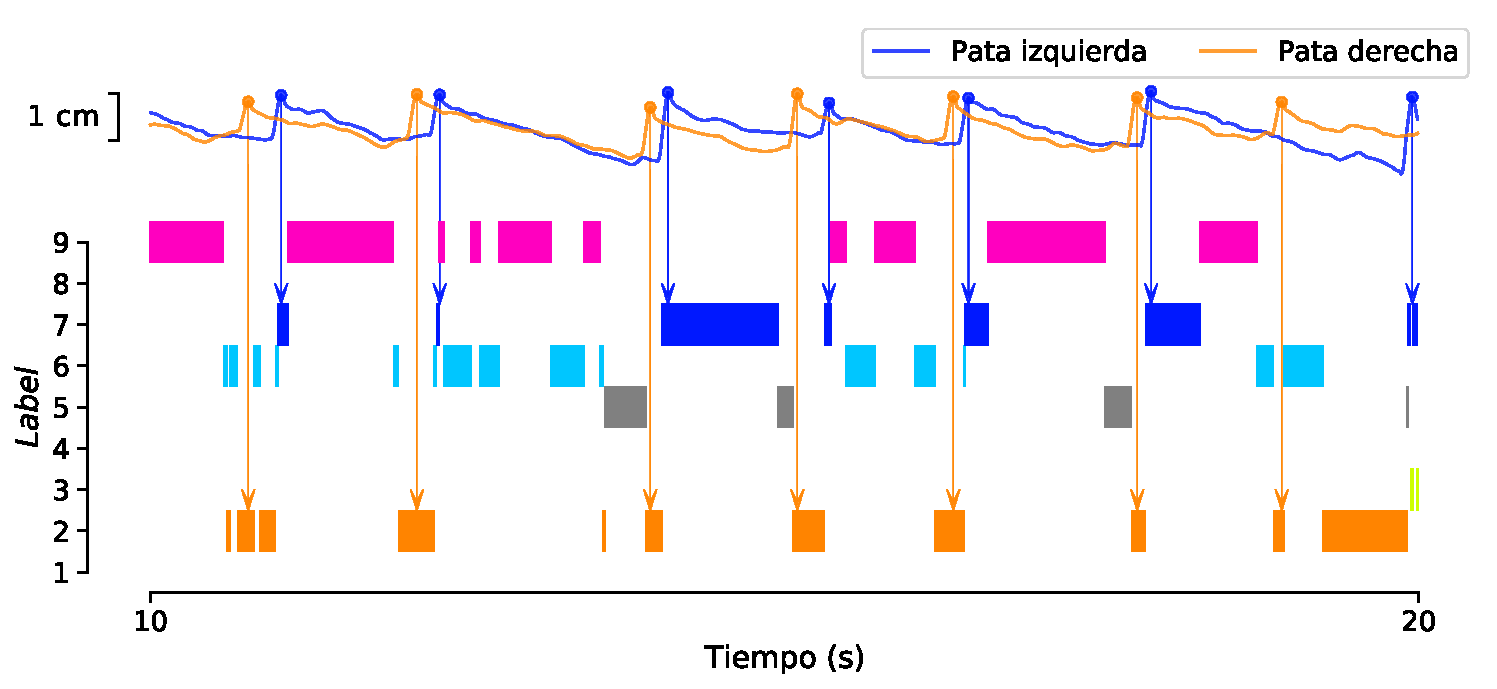
\includegraphics[width=1\linewidth]{figuras/expertos/labels/event_blocks_positions.pdf}
    \caption{Serie temporal típica de \textit{labels}. En la parte superior se muestran la evolución temporal de las coordenadas verticales de las patas izquierda y derecha del ratón. Se indican con círculos los máximos de las posiciones de las patas izquierda y derecha y se trazan flechas hacia los correspondientes \textit{labels} 7 y 2.}
    \label{fig:label_evento_secuencia}
\end{figure}

\section{Representatividad de la clasificación}\label{sec:diversidad}

Una vez que logramos interpretar los \textit{labels} obtenidos, nos preguntamos si la existencia de diferentes poses estaba relacionada a diferentes estrategias comportamentales en animales particulares o si bien eran parte de un repertorio común de poses. Para ello nos preguntamos qué tan representativos son las regiones segmentadas del etograma de la Figura \ref{fig:tsne_labels}. Más precisamente, queremos averiguar si todos los ratones visitan cada una de las regiones del mapa en proporciones similares. La Figura \ref{fig:tsne_mouse_compare} muestra los puntos correspondientes a cada ratón por separado en el etograma (recordemos que en esta práctica se trabajó con un conjunto de $N_{\mathrm{ratones}}=3$ ratones distintos) donde se observa que cada \textit{label} es visitado efectivamente por los tres ratones. 

\begin{figure}[!htbp]
    \centering
    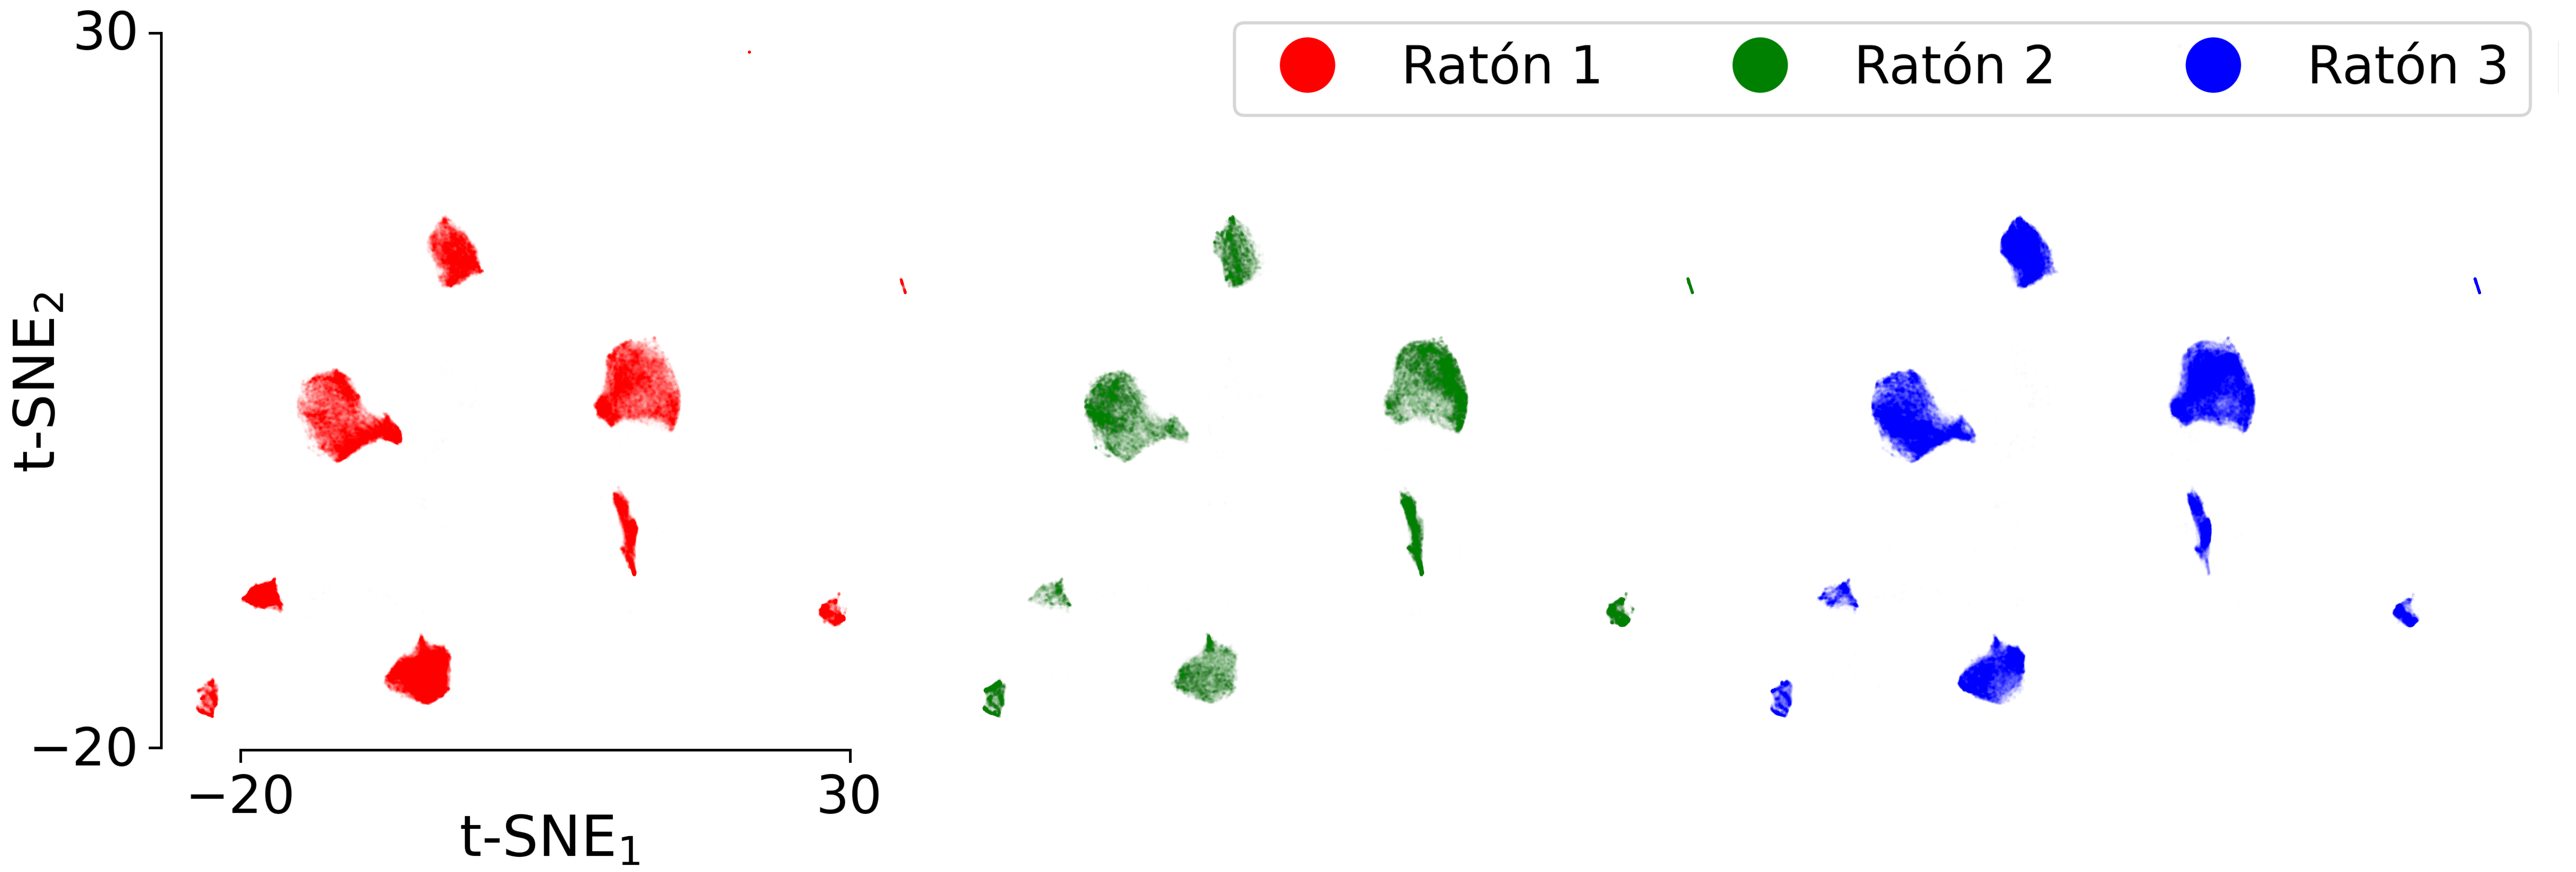
\includegraphics[width=1\linewidth]{figuras/expertos/labels/mouse_compare_tsne.png}
    \caption{Puntos correspondientes a cada ratón por separado en el etograma obtenido.}
    \label{fig:tsne_mouse_compare}
\end{figure}

Con el fin de cuantificar la representatividad de las muestras de ratones de cada región segmentada del etograma calcularemos los índices de diversidad generalizados de orden 2 ${}^{2}D_l$ para cada clase de \textit{label} $l$. Este índice de diversidad ${}^{2}D_l$, también conocido como número efectivo de individuos, es una medida de cuántos ratones diferentes visitan una determinada clase de \textit{label} $l$. Para ello, primero debemos calcular las probabilidades de coincidencia de ratón $\lambda_l$ condicionales a cada clase de \textit{label} $l$. Para una dada clase de \textit{label} $l \in \{ 1, \dots, N_{\mathrm{clases}} \}$ con $N_{\mathrm{clases}} = 9$, se tiene que la probabilidad de que 2 muestras sean del mismo ratón, dado que comparten una misma clase de \textit{label} es
\begin{equation}
    \lambda_l = \sum_{r=1}^{N_{\mathrm{ratones}}} p_{r|l}^2,
\end{equation}
siendo $N_{\mathrm{ratones}}=3$ el número total de ratones distintos observados y $p_{r|l}$ la probabilidad condicional
\begin{equation}
    p_{r|l} = P(\; \text{ratón sea \textit{r}} \;|\; \text{\textit{label} es de clase \textit{l}} \;).
\end{equation}

Dado que la cantidad de observaciones totales para cada ratón no es la misma, vamos a calcular $p_{r|l}$ normalizando la ocurrencia de un \textit{label} de clase $l$ para cada ratón $r$. Para eso, vamos a calcular las probabilidades condicionales
\begin{align}
    p_{l|r} &= P(\; \text{\textit{label} sea de clase \textit{l}} \;|\; \text{ratón es \textit{r}} \;)\\
    &= \frac{n_{l|r}}{N_r},
\end{align}
donde $n_{l|r}$ es el número de observaciones del \textit{label} clase $l$ para el ratón $r$ y $N_r$ es el número total de observaciones del ratón $r$. Note que $\sum_{l=1}^{N_{\mathrm{clases}}} p_{l|r} = 1 \; \forall r$.

La Tabla \ref{tab:diversidad} muestra los valores de las probabilidades condicionales obtenidas $p_{l|r}$. Estos valores muestran que hay variabilidad en la probabilidad de ocurrencia de poses, siendo más frecuentes los \textit{labels} 2, 6, 7 y 9, y el \textit{label} 8 el  menos frecuente. También podemos observar la diferencia inter-animal en la probabilidad de ocurrencia de cada \textit{label}.

A partir de las $p_{l|r}$ podemos calcular las $p_{r|l}$ independientemente de la cantidad total de observaciones de cada ratón, de la siguiente manera
\begin{equation}
    p_{r|l} = p_{l|r} \frac{1}{\sum_{r=1}^{N_{\mathrm{ratones}}} p_{l|r}}.
\end{equation}
Note que estas probabilidades condicionales satisfacen $\sum_{r=1}^{N_{\mathrm{ratones}}} p_{r|l} = 1 \; \forall l$.

Por un lado, si una dada clase de \textit{label} $l$ estuviera ocupada exclusivamente por un sólo tipo de ratón, entonces la probabilidad de coincidencia sería $\lambda_l = 1$. En cambio, si un tipo de \textit{label} $l$ fuera visitado por todos los ratones con probabilidades iguales, entonces la probabilidad de coincidencia de ratones sería $\lambda_l = 1/N_{\mathrm{ratones}} = 1/3$. Además, las probabilidades de coincidencia satisfacen que
\begin{equation}
    \frac{1}{N_{\mathrm{ratones}}} \le \lambda_l \le 1 \; \forall l.
\end{equation}

Esta probabilidad de coincidencia supone que se toman muestras al azar con repetición. Este supuesto puede fallar en caso de contar con pocas observaciones de ratones en cada \textit{label}. En nuestro caso, se cuentan con observaciones totales del orden de $10^5$ para cada ratón y de órdenes entre $10^3$ y $10^4$ para cada tipo de \textit{label} visitado por cada ratón.

Finalmente, a partir de las probabilidades de coincidencia $\lambda_l$ podemos calcular el número efectivo de individuos presentes en cada \textit{label} como
\begin{equation}
    {}^{2}D_l = \frac{1}{\lambda_l}.
\end{equation}

Luego, los valores extremos que puede adoptar el índice de diversidad ${}^{2}D_l$ corresponden a ${}^{2}D_l = 1$ para el caso de una clase de \textit{label} $l$ ocupada por un único tipo de ratón y ${}^{2}D_l = N_{\mathrm{ratones}} = 3$ para el caso de ocupación equiprobable. En la Tabla \ref{tab:diversidad} se indican los valores de los índices de diversidad calculados a partir de esas probabilidades condicionales. Para cada \textit{label} $l$ se resaltaron los valores mayores ${}^{2}D_l = 2.5$. Note que los valores obtenidos satisfacen que $1 \leq {}^{2}D_l \leq 3 \; \forall l$. A partir de este análisis observamos que los \textit{labels} más frecuentes (2, 6, 7 y 9) son visitados similarmente por los tres ratones, pero que también hay \textit{labels} de baja probabilidad y alta representatividad (por ejemplo los \textit{labels} 3 y 5). Por el contrario, el \textit{label} 4 corresponde a una pose que representa con mayor probabilidad al ratón 1.  

\begin{table}[!htbp]
\begin{tabular}{ll|ccccccccc}
\multicolumn{2}{l|}{\textit{label}} & 1 & 2 & 3 & 4 & 5 & 6 & 7 & 8 & 9 \\ \hline
\multirow{3}{*}{$p_{l|r}(\%)$}
& Ratón 1 & 3 & 23 & 4 & 11 & 7 & 22 & 20 & 1 & 11 \\
& Ratón 2 & 6 & 11 & 6 & 2 & 10 & 23 & 30 & 2 & 10 \\
& Ratón 3 & 2 & 13 & 4 & 2 & 6 & 25 & 28 & 2 & 18 \\
\multicolumn{2}{l|}{Diversidad ${}^{2}D_l$}
& 2.46 & \textbf{2.70} & \textbf{2.83} & 1.82 & \textbf{2.83} & \textbf{2.99} & \textbf{2.92} & 2.43 & \textbf{2.78}
\end{tabular}
\caption{Frecuencia condicional $p_{l|r}$ de observar el \textit{label} $l$ del etograma de la Fig. \ref{fig:tsne_labels} con el $r$-ésimo ratón. Valores de diversidad ${}^{2}D_l$ calculados para cada \textit{label} $l$. Se resaltan en negrita aquellos valores de diversidad mayores a ${}^{2}D_l = 2.5$.}
\label{tab:diversidad}
\end{table}

\section{Relación entre el comportamiento y la velocidad del \textit{rotarod}}\label{sec:vel_rotarod}

Las series temporales de \textit{labels} de la Figura \ref{fig:label_evento_secuencia} evidencian que los \textit{labels} tienen diferentes duraciones o tiempos de permanencia. Dado que el paradigma de rotarod utilizado incluye una aceleración positiva constante, nos preguntamos cómo depende la duración de las poses con la velocidad del rotarod y encontramos que las duraciones promedio de los \textit{labels} disminuyen con la velocidad del \textit{rotarod} (Figura \ref{fig:hist_duracion}a). Este resultado está de acuerdo a lo esperado de manera intuitiva: a mayor velocidad de \textit{rotarod}, más rápido cambia de pose el ratón. Para velocidades medias a altas los \textit{labels} 2, 6, 7 y 9 son los de mayor duración (en torno a los 100 ms), mientras que el resto tienen duraciones de entre 30 y 50 ms. Sin embargo, es importante notar que la reducción en la duración de ciertos \textit{labels} no es proporcional con el cambio en velocidad (\textit{labels} 4, 6 y 9) sino que se reduce de manera abrupta indicando un posible cambio en la estrategia comportamental elegida.

Luego, nos preguntamos si es posible distinguir cambios en la estrategia comportamental asociados a diferentes velocidades del rotarod. Para ello, calculamos la probabilidad de ocurrencia de cada \textit{label} a velocidad baja, media o alta independientemente de la duración del mismo. Dado que los \textit{labels} tienen duraciones variables, el estudio de su probabilidad incluyendo la duración podría traer como consecuencia la sobre-representación de los \textit{labels} con mayor duración. En cambio, de la manera propuesta, intentamos poner a los \textit{labels} en pie de igualdad. Para ello definimos secuencias condensadas de \textit{labels} agrupando los \textit{labels} en bloques consecutivos de la misma clase y considerando cada uno de estos bloques como una única observación del \textit{label}. De esta manera resultan secuencias de \textit{labels} sin repeticiones consecutivas de una misma clase, para las que reservaremos la denominación de ``secuencias'', para diferenciarlas de las ``series temporales'' de \textit{labels} de donde provienen. 

Con el fin de entender cómo dependen los \textit{labels} en la secuencia con la velocidad $v$ con la que gira el cilindro del \textit{rotarod}, dividimos las velocidades en tres regímenes, cada uno con cantidades similares de observaciones experimentales. Estos son: velocidades bajas ($v < 13$ rpm), velocidades medias ($13 \leq v < 23$ rpm) y velocidades altas ($v \geq 23$ rpm).

Este análisis nos permitió observar que algunos \textit{labels} aumentan su probabilidad de ocurrencia en la secuencia con la velocidad del rotarod, por ejemplo los \textit{labels} 2, 5 y 7. En cambio, otros \textit{labels} como el 1, 4 y 9 disminuyen su probabilidad (Figura \ref{fig:hist_duracion}b). Estos resultados indican que los animales pasan de una estrategia de locomoción parcialmente sincronizada a bajas velocidades, a una locomoción basada en la alternancia de los miembros inferiores a altas velocidades.  

\begin{figure}[!htbp]
    \centering
    \begin{subfigure}{.49\textwidth}
        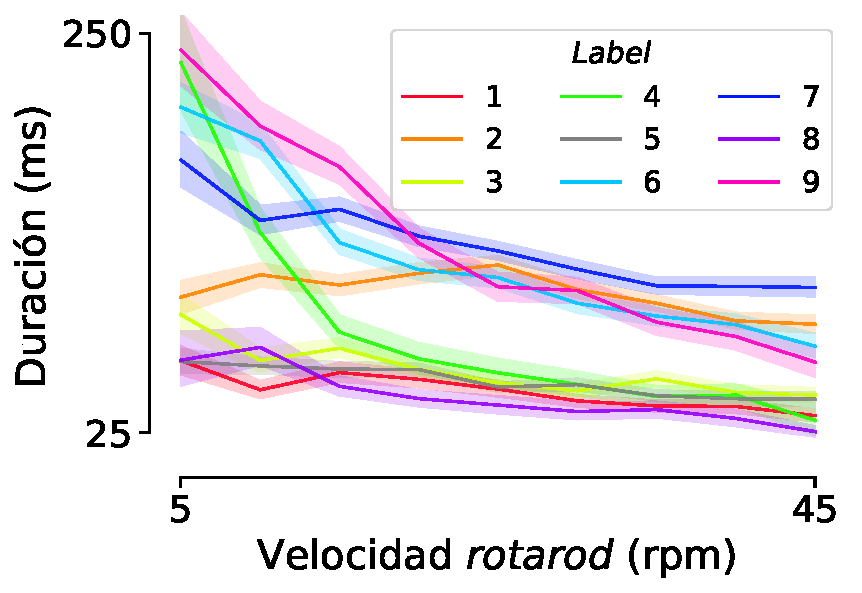
\includegraphics[width=1\textwidth]{figuras/expertos/labels/line_duration_speed.pdf}
        \caption{}
    \end{subfigure}
    \hspace{\fill}
    \begin{subfigure}{.49\textwidth}
        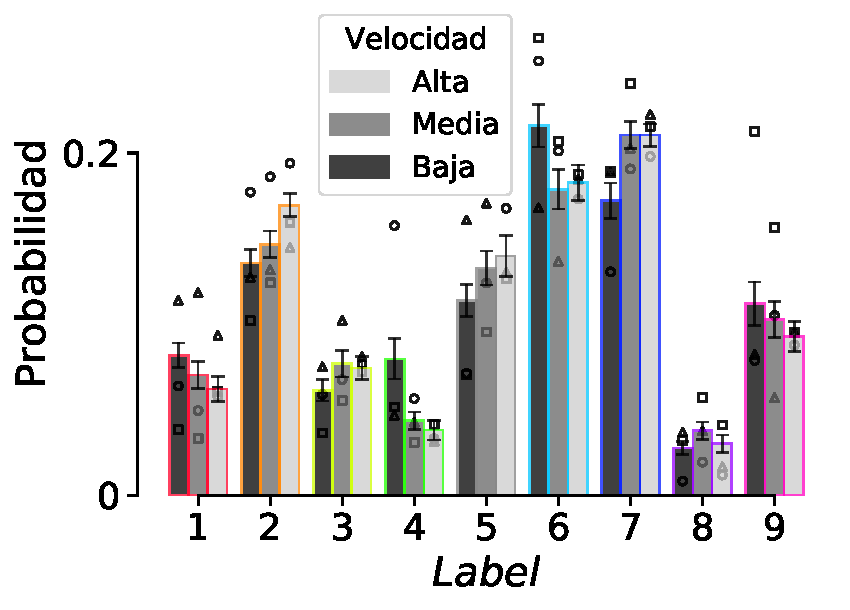
\includegraphics[width=1\textwidth]{figuras/expertos/labels/speed_hist_prob_label.pdf}
        \caption{}
    \end{subfigure}
    \caption{Caracterización de la estadística de las secuencias de \textit{labels} y su dependencia con la velocidad del \textit{rotarod}. (a) Duración promedio de cada \textit{label} en la secuencia, con sus intervalos de confianza. (b) Probabilidad de ocurrencia de cada \textit{label} en la secuencia, bajo tres regímenes de velocidad. Las barras de error representan la desviación estándar del promedio  de las probabilidades al estudiar los \textit{trials rotarod} por separado. Las probabilidades para cada ratón por separado se indican con marcadores vacíos de color negro (círculos: ratón 1, triángulos: ratón 2 y cuadrados: ratón 3). }
    \label{fig:hist_duracion}
\end{figure}

Por último nos interesa investigar la dinámica de las secuencias de \textit{labels}, es decir, qué transiciones de poses ocurren con más frecuencia y cómo cambian estas transiciones con la velocidad del \textit{rotarod}. Esperamos dilucidar de esta manera patrones de locomoción de los ratones durante la ejecución de la tarea.

En primera instancia podemos construir un grafo de transiciones a primer orden, esto es, transiciones entre \textit{labels} inmediatamente consecutivos en la secuencia.  La Figura \ref{fig:trans_grafo_cambios}a muestra que las transiciones entre los \textit{labels} $5 \rightleftarrows 7$, $6 \rightleftarrows 2$, $5 \rightleftarrows 2$ y $6 \rightleftarrows 7$ son las más relevantes en nuestro caso. Casualmente, todas estas son transiciones entre un \textit{label} asociado con dar un paso (2 y 7) y \textit{labels} asociados a poses simétricas (5 y 6). Cabe mencionar que además el \textit{label} 9 (otra pose simétrica) tiene cierta participación, con transiciones destacadas $6 \rightleftarrows 9$ y $7 \rightleftarrows 9$.

Cabe destacar que las posiciones en el grafo de los círculos que representan los \textit{labels} se eligieron de manera tal de reflejar las posiciones de los centros de masa de los \textit{clusters} originales del etograma de la Figura \ref{fig:tsne_labels}. Esto permite visualizar una cierta jerarquía en los \textit{labels} del mapa t-SNE.  Estando los \textit{labels} con transiciones más relevantes (\textit{labels} 2, 5, 6, 7 y 9) ubicados en la parte central del mapa, mientras que los \textit{labels} menos involucrados en las transiciones (\textit{labels} 1, 4, 3 y 8) se encuentran en las periferias del mapa.

Finalmente, la Figura \ref{fig:trans_grafo_cambios}b ilustra los cambios en las probabilidades de transición al aumentar la velocidad del \textit{rotarod}. La figura representa el cambio en las probabilidades de transición para velocidades altas respecto de las probabilidades de transición a velocidades bajas. Note que la diagonal del \textit{heatmap} es cero, pues no estamos considerando auto-transiciones en la secuencia de \textit{labels} (siempre son transiciones entre \textit{labels} distintos). Se observa un aumento en las ocurrencia de transiciones hacia los \textit{labels} 2 y 7 (esto se aprecia en la figura por las columnas con predominancia de color rojo que aparecen en estos \textit{labels}, indicando aumento de probabilidad a altas velocidades). La figura también indica una disminución en la ocurrencia de transiciones hacia los \textit{labels} 4, 6 y 9 a altas velocidades, como se puede apreciar debido a las columnas con predominancia de colores azules sobre los mismos.
En conjunto, estos resultados indican que a mayor velocidad del \textit{rotarod} el ratón selecciona con mayor frecuencia un tipo de locomoción caracterizada por la alternancia de las patas izquierda y derecha, pasando, en algunos casos, por un estado simétrico intermedio.  

\begin{figure}[!htbp]
    \centering
    \begin{subfigure}{.45\textwidth}
        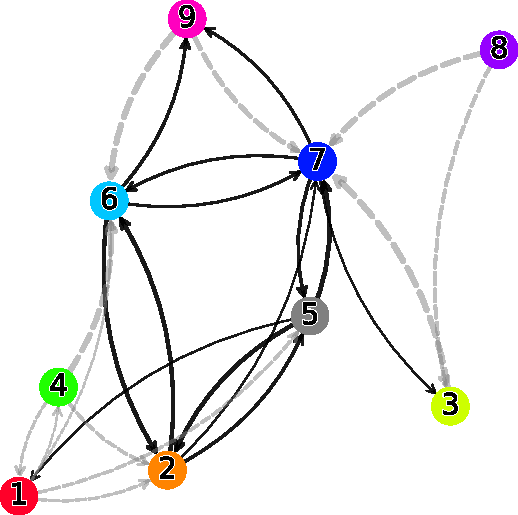
\includegraphics[width=1\textwidth]{figuras/expertos/labels/transition_graph.pdf}
        \caption{}
    \end{subfigure}
    \hspace{\fill}
    \begin{subfigure}{.45\textwidth}
        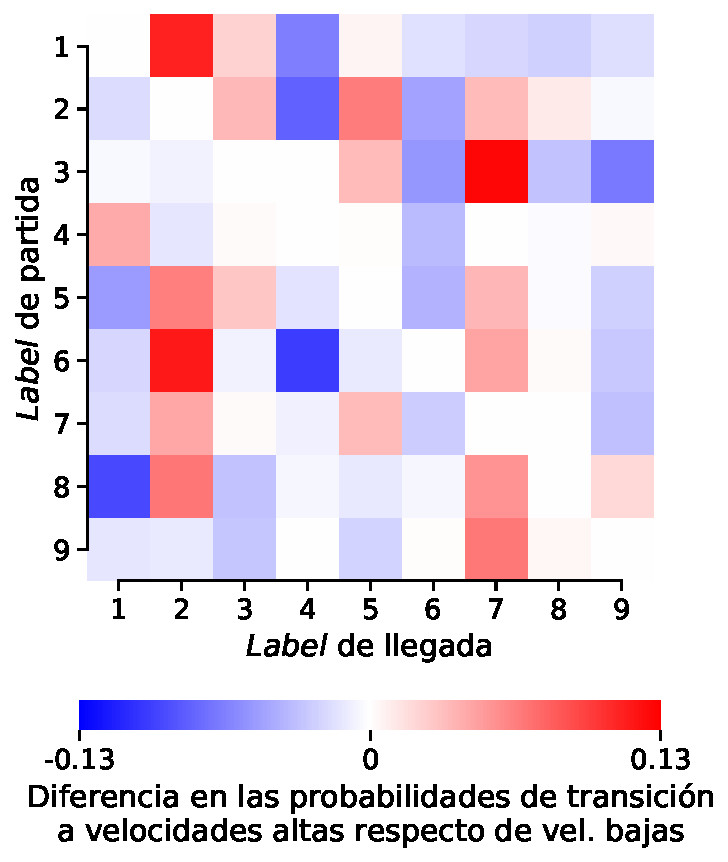
\includegraphics[width=1\textwidth]{figuras/expertos/labels/trans_prob_change.pdf}
        \caption{}
    \end{subfigure}
    \caption{ Transiciones a primer orden en la secuencia de \textit{labels}. (a) Grafo de transiciones. El grosor de las flechas es proporcional a la probabilidad de transición. Las flechas en línea continua negra representan transiciones que parten desde un \textit{label} con probabilidad marginal mayor a $1/N_{\mathrm{clases}} = 0.11$ en la secuencia (para ver las probabilidades marginales de cada \textit{label} referirse a la Figura \ref{fig:hist_duracion}b). Lo opuesto es cierto para las flechas en línea discontinua gris. Solamente se graficaron transiciones que ocurren con probabilidad mayor a $1/ (N_{\mathrm{clases}} - 1) = 0.125$. (b) \textit{Heatmap} indicando las variaciones en la probabilidad de transición a altas velocidades respecto de bajas velocidades. }
    \label{fig:trans_grafo_cambios}
\end{figure}

\section{Dinámica temporal de transiciones entre poses}\label{sec:logo}

El análisis anterior solo permite establecer una relación entre \textit{labels} consecutivos. Para lograr analizar la estructura de nuestras secuencias de \textit{labels} a escalas temporales más largas podemos apoyarnos en el uso de logos de secuencias (\textit{sequence logos}). Estos instrumentos de visualización de secuencias fueron desarrollados por Schneider y Stephens en 1990 \cite{schneider_stephens_logo}, originalmente utilizados para la visualización de secuencias de ácidos nucleicos (secuenciamiento de ADN y ARN) y de aminoácidos (secuenciamiento de proteínas).

En nuestro caso, podemos utilizar logos de secuencias para visualizar transiciones de orden $k$ entre diferentes \textit{labels}. En particular, vamos a condicionar a estas transiciones alrededor de una determinada clase de \textit{label} $l_0 \in \{1, \dots, N_{\mathrm{clases}}\}$, con $N_{\mathrm{clases}} = 9$. Es decir, nos centramos alrededor de cada uno de los \textit{labels} $l$ que satisfagan la condición $l=l_0$ y calcularemos sus probabilidades de transición de orden $k$. Más precisamente, la transición de orden $k=1$ corresponde a calcular las probabilidades de transición desde un determinado \textit{label} $l=l_0$ hacia cualquier otro \textit{label} inmediatamente después, la transición de orden $k=2$ corresponde a estudiar transiciones 2 pasos en el futuro y así sucesivamente. Por su parte, las transiciones de orden negativo ($k<0$) corresponden a estudiar transiciones hacia un determinado \textit{label} $l=l_0$, que provienen desde $|k|$ pasos en el pasado. Identificamos así en un logo de secuencias al orden de transición $k$ con la posición en la secuencia, relativa al lugar donde un \textit{label} adquirió el valor $l_0$. Denotaremos además como $l(k)$ al valor del \textit{label} observado en dicha posición relativa $k$.

Los logos de secuencias son herramientas para graficar el contenido de información de cada posición relativa $k$ de un conjunto de secuencias. En la práctica, para cada clase de \textit{label} $l_0 \in \{1, \dots, N_{\mathrm{clases}}\}$ con $N_{\mathrm{clases}} = 9$, tomaremos todas las secuencias de \textit{labels} observadas centradas en $l(0)=l_0$ y consideraremos transiciones de orden $k$ con $-10 \leq k \leq 10$. Es decir, veremos 10 pasos en el pasado y 10 pasos en el futuro.

Por su parte, el contenido de información es una cantidad proporcional a la entropía de Shannon \cite{shannon_communication, schneider_stephens_logo, schneider_information} asociada a la distribución de probabilidad de \textit{labels} $l(k)$ en una determinada posición relativa $k$ de la secuencia, condicionada por haber observado el valor $l(0)=l_0$. Por simplicidad, denotaremos a esta  distribución de probabilidad condicional como
\begin{equation}
    p_{l', k} = P( \; l(k)=l' \; | \; l(0)=l_0 \;),
\end{equation}
la cual representa la probabilidad de observar el valor de \textit{label} $l'$ en la posición relativa $k$ de la secuencia, dado que observamos el valor de \textit{label} $l_0$ en $k=0$.

Estimaremos estas probabilidades a partir de las frecuencias de \textit{labels} observados, es decir
\begin{equation}
    p_{l, k} = \frac{N_{l, k}}{\sum_{l'=1}^{N_{\mathrm{clases}}} N_{l', k}},
\end{equation}
donde $N_{l, k}$ es el total de \textit{labels} con valor $l$ observados en la $k$-ésima posición relativa del conjunto de secuencias condicionadas por tener el valor de \textit{label} $l_0$ en $k=0$.

A partir de estas distribuciones de probabilidad condicionales podemos calcular la entropía de Shannon, en unidades de \textit{bits}, como
\begin{equation}
    H(k) = - \sum_{l=1}^{N_{\mathrm{clases}}} p_{l, k} \log_2(p_{l, k}),
\end{equation}
donde $H(k)$ nuevamente es la entropía de Shannon de la posición relativa $k$ condicionada a haber observado el valor de \textit{label} $l_0$ en $k=0$.

Finalmente, el contenido de información (eje $y$) de la $k$-ésima posición relativa del conjunto de secuencias condicionadas se calcula a partir de $H(k)$ como
\begin{equation}
    R(k) = \log_2(N_{\mathrm{clases}}) - (H(k) + e(N_{\mathrm{secuencias}})),
\end{equation}
siendo $e(N_{\mathrm{secuencias}})$ un término de corrección \cite{schneider_stephens_logo} que depende de la cantidad total de secuencias muestreadas $N_{\mathrm{secuencias}}$
\begin{equation}
    e(N_{\mathrm{secuencias}}) = \frac{1}{\ln(2)} \frac{N_{\mathrm{clases}} - 1}{2 N_{\mathrm{secuencias}}}.
\end{equation}

El valor mínimo que puede adoptar el contenido de información es $R(k) = 0$. Este valor corresponde a tener una distribución de probabilidad uniforme de \textit{labels} en la $k$-ésima posición, es decir, todos las clases de \textit{labels} tienen la misma probabilidad. El máximo valor que puede adoptar el contenido de información es $R(k) = \log_2(N_{\mathrm{clases}}) = 3.17$ \textit{bits}. Por su parte, este valor corresponde a tener una distribución de probabilidad \textit{labels} completamente determinista, es decir, una única clase de \textit{label} con probabilidad uno y todas las demás con probabilidad cero. Esto ocurre siempre en la posición $k=0$, pues condicionamos nuestros logos de secuencias a cumplir con $l(0) = l_0$. Por último, el contenido de información satisface que $0 \leq R(k) \leq 3.17$ \textit{bits} $\forall k$.

Finalmente, en la gráfica de un logo de secuencias, se le asigna a cada clase de \textit{label} $l$ una fracción del contenido de información $R(k)$ en proporción a su probabilidad condicional $p_{l,k}$
\begin{equation}
    R_{l,k} = p_{l,k} R(k).
\end{equation}

La Figura \ref{fig:logos} muestra los logos de secuencias condicionales, centradas alrededor de cada uno de los \textit{labels} obtenidos de la segmentación del mapa de comportamientos. Para cada posición relativa en la secuencia, la clase de \textit{label} más probable se coloca en la base y la menos probable en la cima de la columna. Note que el \textit{label} en la posición relativa central $k=0$ tiene siempre un contenido de información máximo $R(0) = 3.17$ \textit{bits}, pues estamos estudiando secuencias condicionadas de esa manera. Note además que el \textit{label} central en $k=0$ está dentro de un recuadro de línea discontinua y su altura no está a escala. Estos logos de secuencias exponen patrones alternantes recurrentes, que involucran en todos los casos al \textit{label} central, junto con uno o dos \textit{labels} más probables en la alternancia. Puede observarse que los \textit{labels} más involucrados en los patrones alternantes de los demás son los \textit{labels} número 7, 6, 5 y 2.

Además, en la Figura \ref{fig:logos} pueden observarse oscilaciones en el valor total del contenido de información, especialmente en los logos centrados en los \textit{labels} 6, 7 y 9. Recordemos que el valor de $R(k)$, el contenido de información de la posición relativa $k$, baja cuando la distribución de probabilidad de los \textit{labels} en esa posición se vuelve más uniforme (probabilidades iguales) y aumenta cuando la distribución se vuelve más concentrada (pocos \textit{labels} mucho más probables que los demás). Por lo tanto, en las oscilaciones del contenido de información, los valles representan posiciones con \textit{labels} indeterminados y los picos están asociados a posiciones donde predominan algunos \textit{labels} sobre los demás.

\begin{landscape}
\begin{figure}[!htbp]
\begin{minipage}{0.5\linewidth}
    \centering
    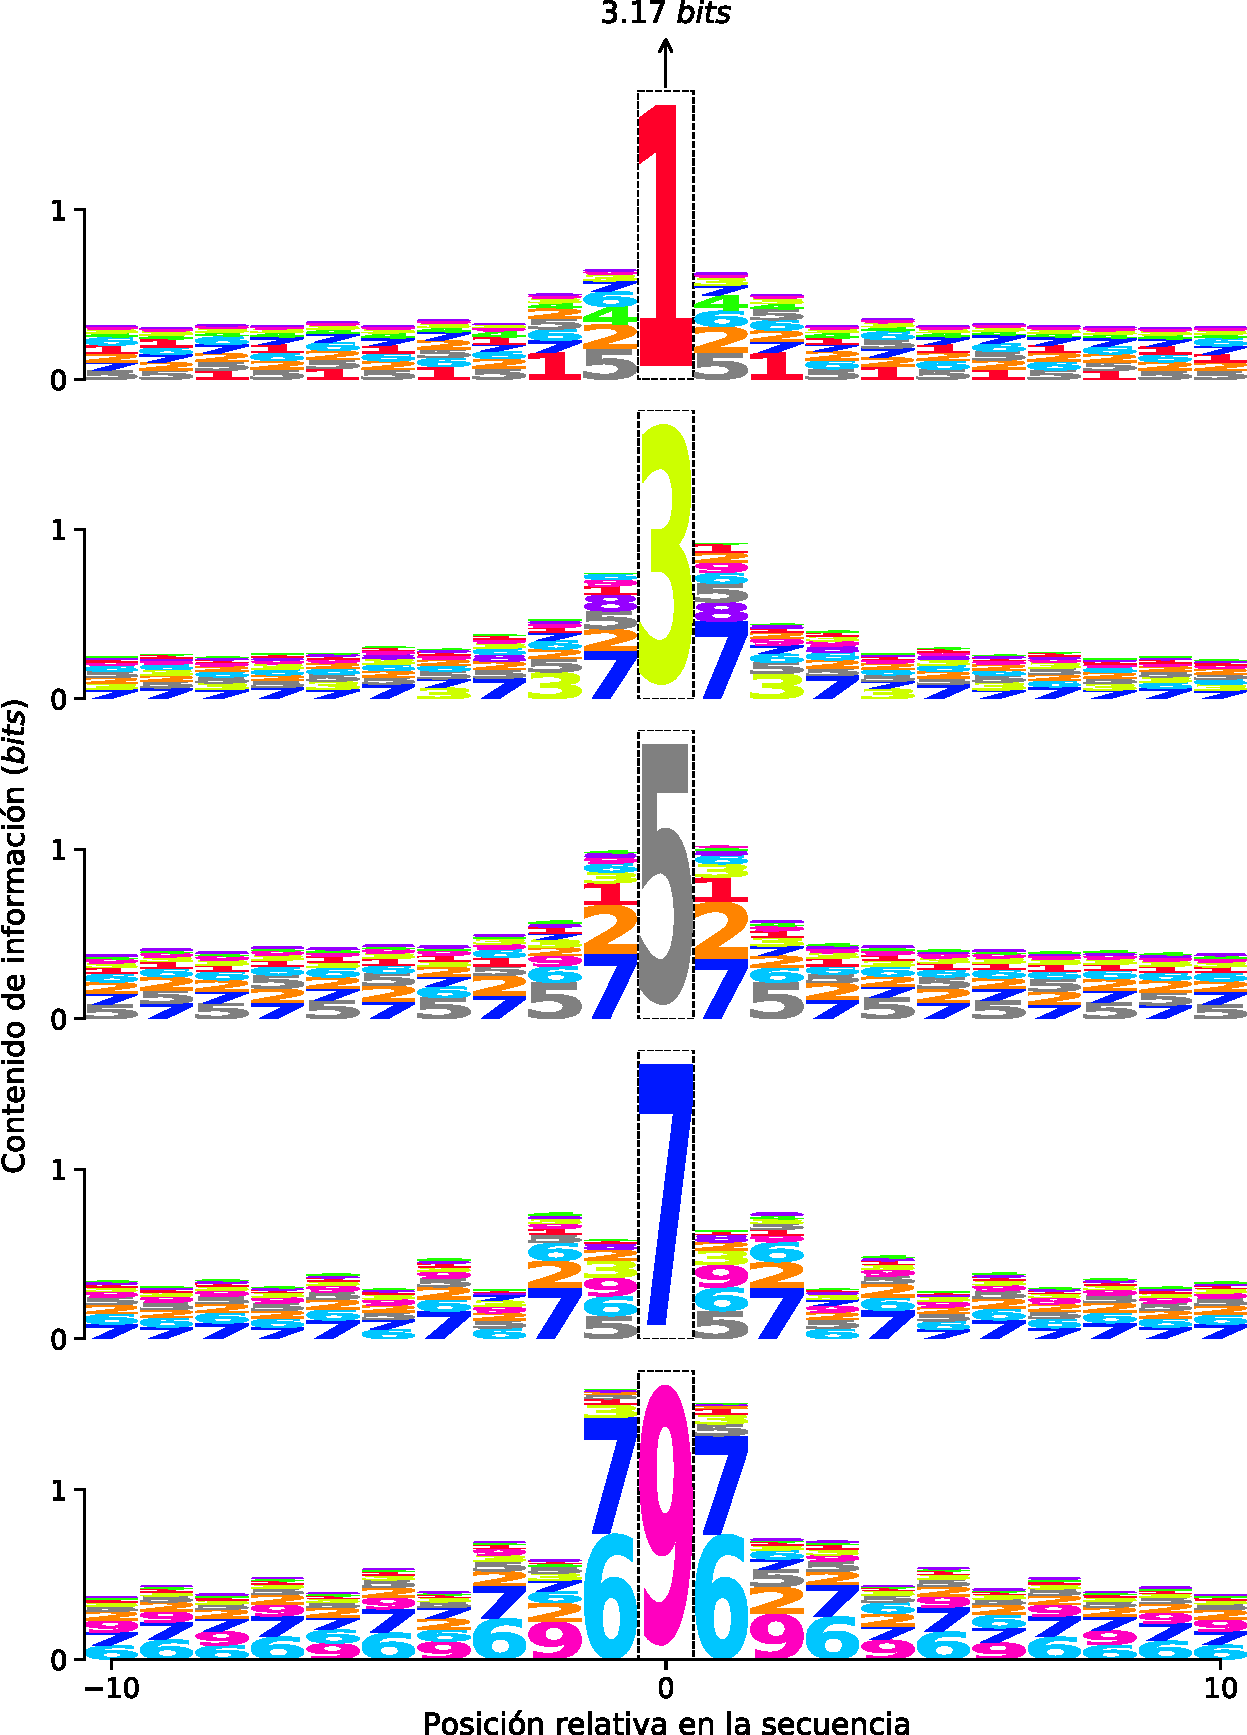
\includegraphics[width=.9\linewidth]{figuras/expertos/logos/conditional_logos_odd.pdf}
\end{minipage}
\begin{minipage}{0.42\linewidth}
    \centering
    \vspace{-0.25em}
    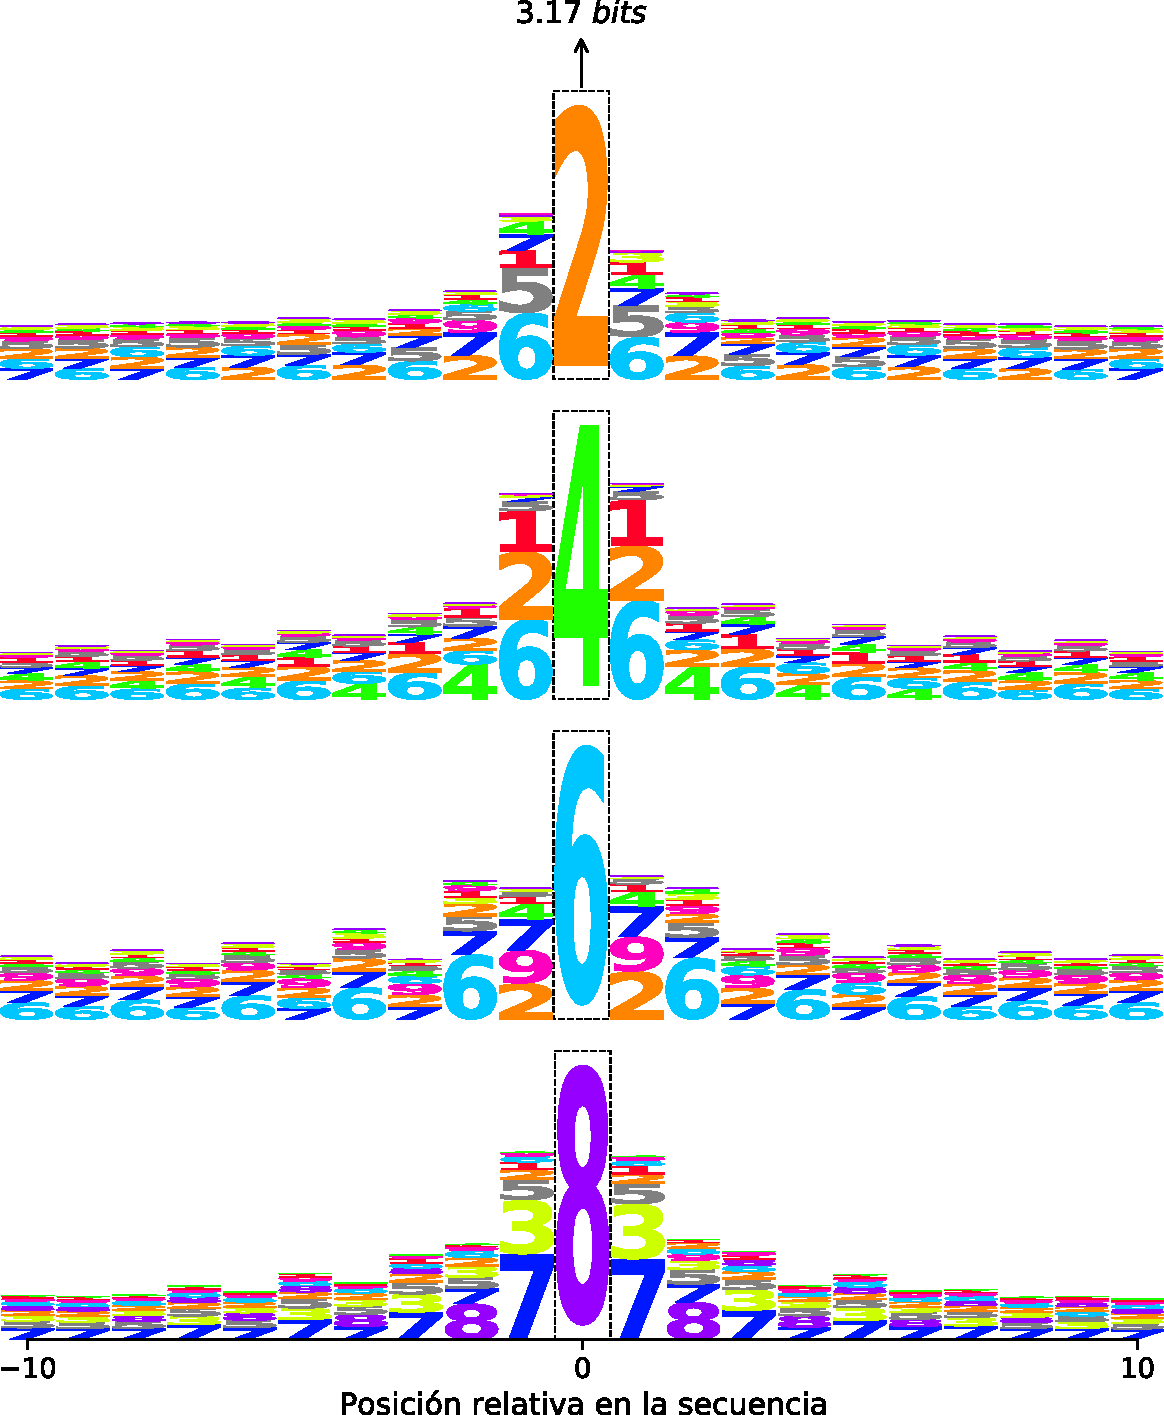
\includegraphics[width=1\linewidth]{figuras/expertos/logos/conditional_logos_even.pdf}
    \caption{Logos de secuencias condicionales, centrados alrededor de cada una de las clases de \textit{label}. La altura de cada \textit{label} en una determinada columna en la posición relativa $k$ es proporcional a la probabilidad de transición de orden $k$ relativa al \textit{label} central.}
    \label{fig:logos}
\end{minipage}
\end{figure}
\end{landscape}
